%Sexto ejercicio.
\documentclass{standalone}
\usepackage[utf8x]{inputenc}
\usepackage[T1]{fontenc}
\usepackage{PTSansNarrow}
\usepackage[usenames,dvipsnames,x11names,table,svgnames]{xcolor}
\usepackage{tikz}
\usetikzlibrary{babel,calc}
\begin{document}

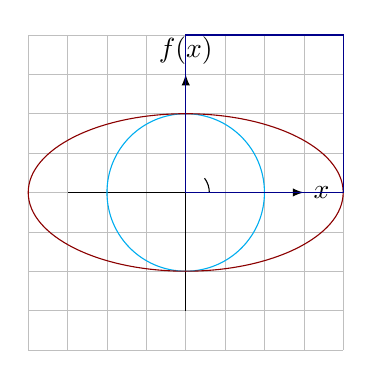
\begin{tikzpicture}
\def\t{37}
\draw[gray!50, very thin, xstep = .5, ystep = .5] (-2, -2) grid (2,2);
%\clip (.15, 0);
%\clip (0, .5cm) circle ;
%\clip(.15, 0) circle (.5cm); %Investigar el uso de clip.
\draw (3mm, 0) arc[start angle = 0, end angle = \t, radius =.3];
\draw[>=latex, ->] (-1.5,0) -- (1.5, 0) node[right] {$x$};
\draw[>=latex, ->] (0, -1.5) -- (0, 1.5) node[above] {$f(x)$};
\draw[cyan](0,0) circle[radius =1];
\draw[DarkRed] (0,0) ellipse[x radius =2, y radius =1];
\draw[DarkBlue] (0,0) rectangle (2,2);
\end{tikzpicture}

\end{document}